% Figure: Data Augmentation Results
% Effect of augmentation on model performance

\documentclass[border=5pt]{standalone}
\usepackage[utf8]{inputenc}
\usepackage{pgfplots}
\usepackage{tikz}
\usepackage{helvet}
\usepackage[T1]{fontenc}

\pgfplotsset{
    width=14cm,
    height=7cm,
    compat=1.18,
}

\begin{document}
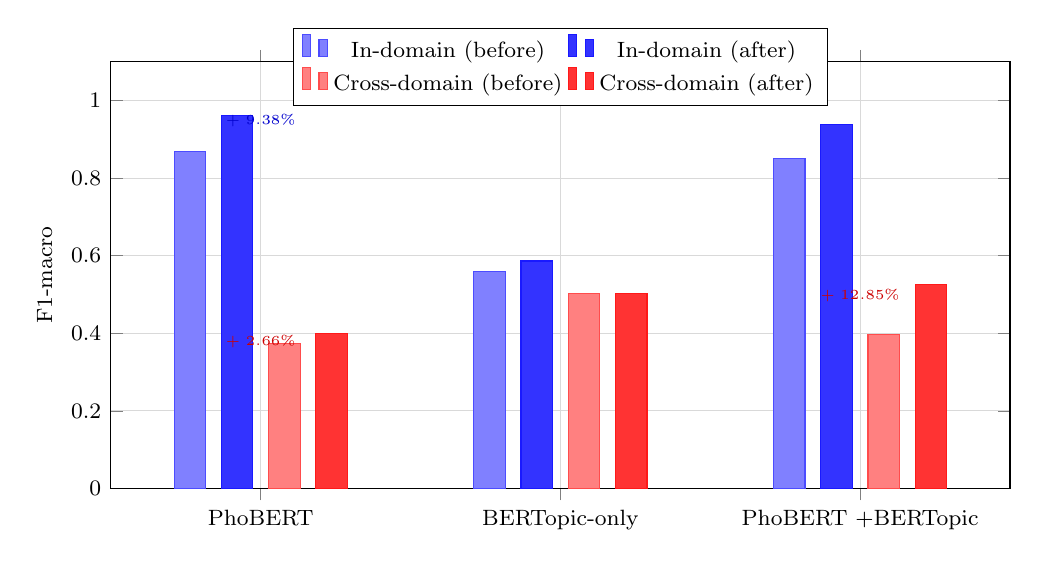
\begin{tikzpicture}
\begin{axis}[
    width=13cm,
    height=7cm,
    ybar=0.2cm,
    bar width=0.4cm,
    enlarge x limits=0.25,
    ymin=0, ymax=1.1,
    ylabel={F1-macro},
    ylabel style={font=\footnotesize},
    tick label style={font=\fontsize{8}{9}\selectfont},
    grid=major,
    grid style={gray!30},
    ytick distance=0.2,
    legend style={
        at={(0.5,1.08)},
        anchor=north,
        legend columns=2,
        font=\footnotesize
    },
    cycle list={
        {fill=blue!50,draw=blue!70},
        {fill=blue!80,draw=blue!90},
        {fill=red!50,draw=red!70},
        {fill=red!80,draw=red!90},
    },
    xtick=data,
    xticklabels={
        {PhoBERT},
        {BERTopic-\\only},
        {PhoBERT +\\BERTopic}
    },
]

% In-domain before
\addplot coordinates {
    (1, 0.8681)
    (2, 0.5599)
    (3, 0.8504)
};
\addlegendentry{In-domain (before)}

% In-domain after
\addplot coordinates {
    (1, 0.9619)
    (2, 0.5864)
    (3, 0.9377)
};
\addlegendentry{In-domain (after)}

% Cross-domain before
\addplot coordinates {
    (1, 0.3727)
    (2, 0.5030)
    (3, 0.3977)
};
\addlegendentry{Cross-domain (before)}

% Cross-domain after
\addplot coordinates {
    (1, 0.3993)
    (2, 0.5022)
    (3, 0.5262)
};
\addlegendentry{Cross-domain (after)}

% Annotations for improvements
\node[anchor=north, font=\tiny, blue!80!black] at (axis cs:1,0.99) {$+\;9.38\%$};
\node[anchor=north, font=\tiny, red!80!black] at (axis cs:1,0.42) {$+\;2.66\%$};

\node[anchor=north, font=\tiny, red!80!black] at (axis cs:3,0.54) {$+\;12.85\%$};

\end{axis}
\end{tikzpicture}
\end{document}
